\documentclass[aspectratio=169,14pt]{beamer}

% ── Theme ──────────────────────────────────────────────
\usetheme{metropolis}
\usepackage{appendixnumberbeamer}
\usepackage{booktabs}
\usepackage{amsmath,amssymb}
\usepackage{graphicx}
\usepackage{tikz}
\usetikzlibrary{arrows.meta,positioning,calc}
\usepackage{listings}
\usepackage{xcolor}

% ── Colors ─────────────────────────────────────────────
\definecolor{geccoBlue}{RGB}{25,50,95}
\definecolor{geccoAccent}{RGB}{50,130,200}
\definecolor{geccoHighlight}{RGB}{220,80,60}
\definecolor{geccoGreen}{RGB}{40,160,80}
\definecolor{codeBg}{RGB}{245,245,250}
\definecolor{haskellPurple}{RGB}{90,50,140}
\definecolor{rustOrange}{RGB}{180,80,20}

\setbeamercolor{frametitle}{bg=geccoBlue,fg=white}
\setbeamercolor{title}{fg=white}
\setbeamercolor{alerted text}{fg=geccoHighlight}
\setbeamercolor{progress bar}{fg=geccoAccent}

% ── Code listings ──────────────────────────────────────
\lstset{
  basicstyle=\ttfamily\scriptsize,
  backgroundcolor=\color{codeBg},
  frame=single,
  framerule=0pt,
  breaklines=true,
  columns=fullflexible,
  keepspaces=true,
}

% ── Figure paths ───────────────────────────────────────
\graphicspath{
  {../gecco-camera-ready/}
  {../gecco-camera-ready/supplementary/experiments/plots/}
  {../lyra-first-draft-gecco/}
  {../experiments/plots/}
  {../EUMAS/}
  {../EUMAS/may11/figures/}
}

% ── Meta ───────────────────────────────────────────────
\title{Composition Determines Diversity}
\subtitle{Categorical Fingerprints of Genetic Algorithms}
\author{Robin Langer \and Claudius Turing \and Lyra Vega}
\institute{GECCO 2026 \quad $\cdot$ \quad San Jos\'{e}, Costa Rica}
\date{July 13--17, 2026}

\begin{document}

% ═══════════════════════════════════════════════════════
% SECTION 1: Opening Hook (2 min)
% ═══════════════════════════════════════════════════════

% ── Slide 1: Title ─────────────────────────────────────
{
\setbeamercolor{background canvas}{bg=geccoBlue}
\begin{frame}[plain]
  \vfill
  \begin{center}
    {\Huge\bfseries\color{white} Composition Determines Diversity}\\[12pt]
    {\large\color{geccoAccent} Categorical Fingerprints of Genetic Algorithms}\\[24pt]
    {\normalsize\color{white} Robin Langer \quad $\cdot$ \quad Claudius Turing \quad $\cdot$ \quad Lyra Vega}\\[8pt]
    {\small\color{gray!60} GECCO 2026 \quad $\cdot$ \quad San Jos\'{e}, Costa Rica}
  \end{center}
  \vfill
  \begin{center}
    {\small\color{geccoAccent}\itshape ``How you wire your islands matters more than what you evolve''}
  \end{center}
  \vfill
\end{frame}
}

% ── Slide 2: The Surprising Claim ★ AHA MOMENT ────────
\begin{frame}{The Surprising Claim}
  \begin{center}
    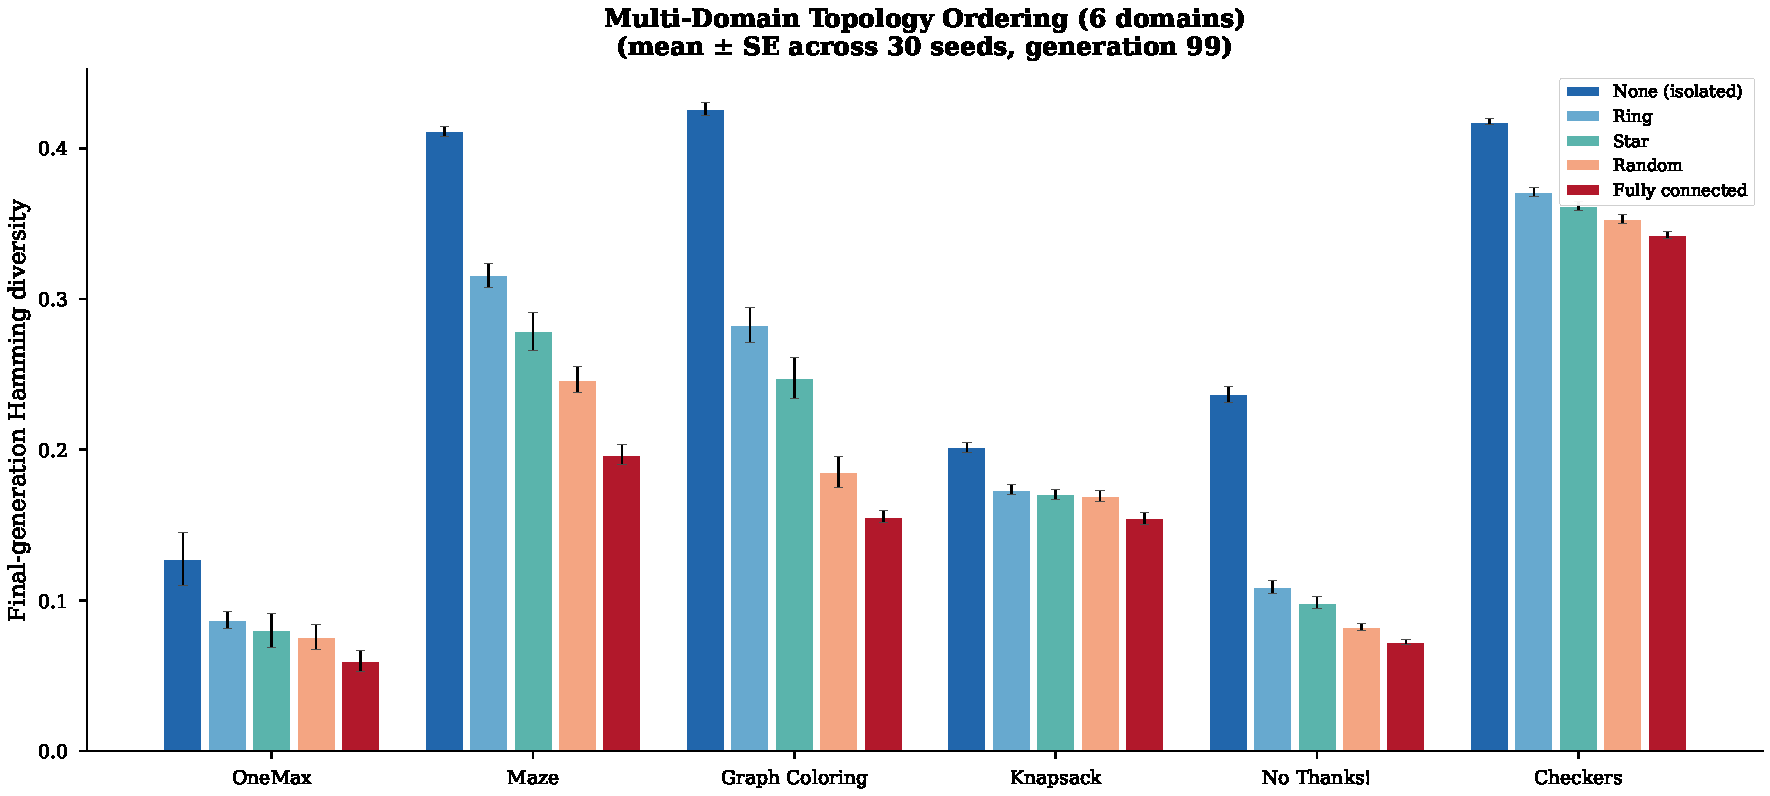
\includegraphics[width=0.85\textwidth]{multi_domain_topology_ordering.pdf}
  \end{center}
  \vspace{-6pt}
  \begin{columns}[T]
    \column{0.33\textwidth}
    \centering\small
    \alert{$W = 1.0$}\\
    Perfect concordance
    \column{0.33\textwidth}
    \centering\small
    \alert{$p = 0.00008$}\\
    Not noise
    \column{0.33\textwidth}
    \centering\small
    \alert{23.9$\times$}\\
    Topology $\gg$ domain
  \end{columns}
  \note{Show this result FIRST, then spend the talk explaining why.
    Migration topology explains 23.9x more variance in diversity than domain choice.
    The ordering none > ring > star > random > FC holds with Kendall's W = 1.0
    across 6 completely unrelated domains. p = 0.00008.}
\end{frame}

% ── Slide 3: Why Should You Care? ─────────────────────
\begin{frame}{Why Should You Care?}
  \begin{columns}[T]
    \column{0.45\textwidth}
    {\color{gray}\small What practitioners tune}\\[6pt]
    \begin{itemize}
      \item Crossover type
      \item Mutation rate
      \item Population size
      \item Selection pressure
    \end{itemize}
    \column{0.1\textwidth}
    \centering\vspace{30pt}
    {\Huge\color{geccoHighlight} $\ll$}
    \column{0.45\textwidth}
    {\color{geccoAccent}\small\bfseries What actually determines diversity}\\[6pt]
    \begin{itemize}
      \item \textbf{Composition structure}
      \item \textbf{Migration topology}
      \item[$\to$] Choose topology FIRST
    \end{itemize}
  \end{columns}
  \vfill
  {\small Three practical recommendations at the end of this talk.}
  \note{Practitioners spend weeks tuning operators; topology is chosen once and forgotten.
    Our result: choose topology FIRST --- it dominates everything else.}
\end{frame}

% ═══════════════════════════════════════════════════════
% SECTION 2: The Categorical Framework (4 min)
% ═══════════════════════════════════════════════════════
\section{The Categorical Framework}

% ── Slide 4: Hidden Composition ───────────────────────
\begin{frame}[fragile]{The Problem: Hidden Composition}
  Every GA composes operators:
  \[
    \texttt{select} \;\to\; \texttt{crossover} \;\to\; \texttt{mutate} \;\to\; \texttt{replace}
  \]

  \vspace{6pt}
  In imperative code, this pipeline is \alert{invisible}:
  \vspace{4pt}

  \lstset{basicstyle=\ttfamily\fontsize{7}{8.5}\selectfont,
    keywordstyle=\color{rustOrange}\bfseries,
    commentstyle=\color{gray},
    morekeywords={for,in,let}}
  \begin{lstlisting}
for gen in 0..max_gens {
    let parent_a = tournament_select(&pop, &fitness, rng);
    let parent_b = tournament_select(&pop, &fitness, rng);
    let (child_a, child_b) = crossover(parent_a, parent_b, cx_rate, rng);
    let child_a = mutate(child_a, mut_rate, rng);
    let child_b = mutate(child_b, mut_rate, rng);
    // ... 60+ more lines of manual sequencing
}
  \end{lstlisting}

  \vspace{4pt}
  {\small Cannot formally ask: \emph{``does this composition preserve a property?''}}
  \note{Every GA composes operators but in imperative code this composition is
    invisible --- buried in loops. Cannot formally reason about composition.}
\end{frame}

% ── Slide 5: Making Composition Explicit ★ AHA MOMENT ─
\begin{frame}[fragile]{Making Composition Explicit}
  \begin{columns}[T]
    \column{0.55\textwidth}
    {\color{haskellPurple}\bfseries Kleisli composition (6 lines)}
    \lstset{basicstyle=\ttfamily\fontsize{8}{10}\selectfont,
      keywordstyle=\color{haskellPurple}\bfseries,
      morekeywords={evolve,tournamentSelect,crossover,mutate,evaluate}}
    \begin{lstlisting}
evolve :: Pop a -> Evo (Pop a)
evolve =
    tournamentSelect
  >>> crossover
  >>> mutate
  >>> evaluate
    \end{lstlisting}

    \vspace{8pt}
    {\small Operators typed as\\
    \quad $f : \mathsf{Pop}\,a \to M(\mathsf{Pop}\,a)$\\[4pt]
    Same type in, same type out.\\
    \alert{Composable by construction.}}

    \column{0.45\textwidth}
    {\color{rustOrange}\bfseries Imperative (75 lines)}\\[4pt]
    {\footnotesize Manual sequencing, index arithmetic, explicit effect threading, interleaved concerns\ldots}

    \vspace{12pt}
    \begin{center}
    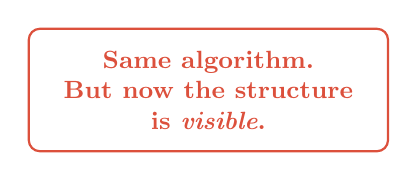
\begin{tikzpicture}
      \node[draw=geccoHighlight,thick,rounded corners,inner sep=8pt,
            text width=4cm,align=center,font=\small\bfseries\color{geccoHighlight}]
        {Same algorithm.\\But now the structure\\is \emph{visible}.};
    \end{tikzpicture}
    \end{center}
  \end{columns}
  \note{AHA: Six lines. Same algorithm. But now the structure is VISIBLE.
    Kleisli arrows let us compose with effects handled automatically.}
\end{frame}

% ── Slide 6: Three Composition Levels ─────────────────
\begin{frame}{Three Composition Levels}
  \begin{center}
  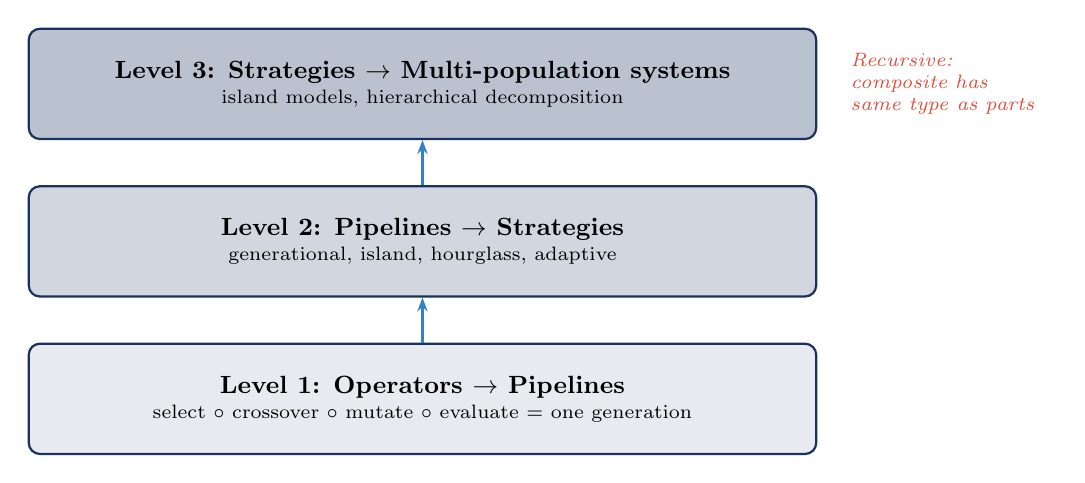
\begin{tikzpicture}[
    level/.style={draw=geccoBlue,thick,rounded corners,minimum width=10cm,
                  minimum height=1.4cm,align=center,font=\small},
    arr/.style={-{Stealth[length=5pt]},thick,geccoAccent}
  ]
    \node[level,fill=geccoBlue!10] (L1) at (0,0)
      {\textbf{Level 1: Operators $\to$ Pipelines}\\[-2pt]
       \scriptsize select $\circ$ crossover $\circ$ mutate $\circ$ evaluate = one generation};
    \node[level,fill=geccoBlue!20] (L2) at (0,2)
      {\textbf{Level 2: Pipelines $\to$ Strategies}\\[-2pt]
       \scriptsize generational, island, hourglass, adaptive};
    \node[level,fill=geccoBlue!30] (L3) at (0,4)
      {\textbf{Level 3: Strategies $\to$ Multi-population systems}\\[-2pt]
       \scriptsize island models, hierarchical decomposition};

    \draw[arr] (L1) -- (L2);
    \draw[arr] (L2) -- (L3);

    \node[right=0.3cm of L3,font=\scriptsize\itshape\color{geccoHighlight},
          text width=2.5cm,align=left] {Recursive:\\composite has\\same type as parts};
  \end{tikzpicture}
  \end{center}
  \note{Three levels of composition. The key insight: at every level,
    the composite has the same type as its parts --- recursive composability.}
\end{frame}

% ── Slide 7: Domain Invariance ────────────────────────
\begin{frame}{Domain Invariance}
  \begin{center}
  {\small Pipeline shape is \alert{identical} across all domains.}
  \end{center}

  \vspace{6pt}
  \begin{center}
  \begin{tabular}{@{}lcc@{}}
    \toprule
    \textbf{Component} & \textbf{Changes?} & \textbf{Why} \\
    \midrule
    Genome type $a$ & \checkmark & Problem-specific \\
    Fitness function & \checkmark & Problem-specific \\
    \midrule
    Pipeline shape & $\times$ & Categorical structure \\
    Composition laws & $\times$ & Kleisli category \\
    Strategy patterns & $\times$ & Functor composition \\
    Migration structure & $\times$ & Graph topology \\
    \bottomrule
  \end{tabular}
  \end{center}

  \vfill
  {\small\itshape Category theory predicts this: structure lives in \alert{arrows}, not objects.}
  \note{Only genome type and fitness function change. Everything about the
    composition structure is invariant. Category theory predicts this.}
\end{frame}

% ═══════════════════════════════════════════════════════
% SECTION 3: The Experiment (3 min)
% ═══════════════════════════════════════════════════════
\section{Experimental Setup}

% ── Slide 8: Six Domains ──────────────────────────────
\begin{frame}{Six Domains}
  \begin{columns}[T]
    \column{0.5\textwidth}
    \begin{enumerate}
      \item \textbf{OneMax}\\[-2pt]
            {\scriptsize Trivial unimodal}
      \item \textbf{Maze Generation}\\[-2pt]
            {\scriptsize Binary, multi-objective}
      \item \textbf{Graph Coloring}\\[-2pt]
            {\scriptsize Constraint satisfaction}
    \end{enumerate}
    \column{0.5\textwidth}
    \begin{enumerate}\setcounter{enumi}{3}
      \item \textbf{Knapsack}\\[-2pt]
            {\scriptsize Epistatic interactions}
      \item \textbf{No Thanks!}\\[-2pt]
            {\scriptsize Co-evolutionary, \alert{no fixed landscape}}
      \item \textbf{Checkers}\\[-2pt]
            {\scriptsize Intransitive fitness}
    \end{enumerate}
  \end{columns}

  \vspace{12pt}
  \begin{center}
    {\small Chosen to span: landscape structure $\times$ representation type $\times$ constraint type}
  \end{center}
  \note{Six completely unrelated domains spanning: trivial to NP-hard,
    fixed to co-evolutionary landscapes, binary to real-valued.}
\end{frame}

% ── Slide 9: Experimental Setup ───────────────────────
\begin{frame}{Experimental Setup}
  \begin{columns}[T]
    \column{0.5\textwidth}
    \begin{itemize}
      \item 5 islands $\times$ 16 individuals
      \item 100 generations
      \item 5 topologies
      \item 30 seeds per condition
      \item \textbf{900 runs total}
    \end{itemize}

    \vspace{8pt}
    {\small Diversity = normalized pairwise\\Hamming/Euclidean distance}

    \column{0.5\textwidth}
    \begin{center}
    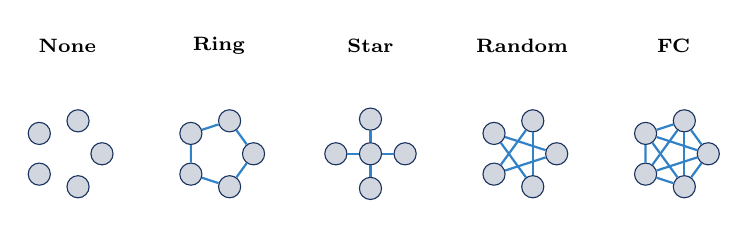
\begin{tikzpicture}[scale=0.55,
      node/.style={circle,draw=geccoBlue,fill=geccoBlue!20,
                   minimum size=8pt,inner sep=0pt}]
      % None
      \node[font=\scriptsize\bfseries] at (0,2.5) {None};
      \foreach \i in {1,...,5} {
        \node[node] (n\i) at ({72*\i-72}:0.8) {};
      }

      % Ring
      \begin{scope}[xshift=3.5cm]
        \node[font=\scriptsize\bfseries] at (0,2.5) {Ring};
        \foreach \i in {1,...,5} {
          \node[node] (r\i) at ({72*\i-72}:0.8) {};
        }
        \foreach \i/\j in {1/2,2/3,3/4,4/5,5/1} {
          \draw[geccoAccent,thick] (r\i) -- (r\j);
        }
      \end{scope}

      % Star
      \begin{scope}[xshift=7cm]
        \node[font=\scriptsize\bfseries] at (0,2.5) {Star};
        \node[node] (sc) at (0,0) {};
        \foreach \i in {1,...,4} {
          \node[node] (s\i) at ({90*\i-90}:0.8) {};
          \draw[geccoAccent,thick] (sc) -- (s\i);
        }
      \end{scope}

      % Random
      \begin{scope}[xshift=10.5cm]
        \node[font=\scriptsize\bfseries] at (0,2.5) {Random};
        \foreach \i in {1,...,5} {
          \node[node] (d\i) at ({72*\i-72}:0.8) {};
        }
        \draw[geccoAccent,thick] (d1) -- (d3);
        \draw[geccoAccent,thick] (d2) -- (d5);
        \draw[geccoAccent,thick] (d1) -- (d4);
        \draw[geccoAccent,thick] (d3) -- (d5);
        \draw[geccoAccent,thick] (d2) -- (d4);
      \end{scope}

      % FC
      \begin{scope}[xshift=14cm]
        \node[font=\scriptsize\bfseries] at (0,2.5) {FC};
        \foreach \i in {1,...,5} {
          \node[node] (f\i) at ({72*\i-72}:0.8) {};
        }
        \foreach \i in {1,...,5} {
          \foreach \j in {\i,...,5} {
            \draw[geccoAccent,thick] (f\i) -- (f\j);
          }
        }
      \end{scope}
    \end{tikzpicture}
    \end{center}
  \end{columns}
  \note{5 islands x 16 individuals, 100 generations, 30 seeds per (topology, domain)
    = 900 runs total. Five topologies from disconnected to fully connected.}
\end{frame}

% ── Slide 10: Topologies + Lambda_2 ──────────────────
\begin{frame}{Five Topologies: Algebraic Connectivity}
  \begin{center}
  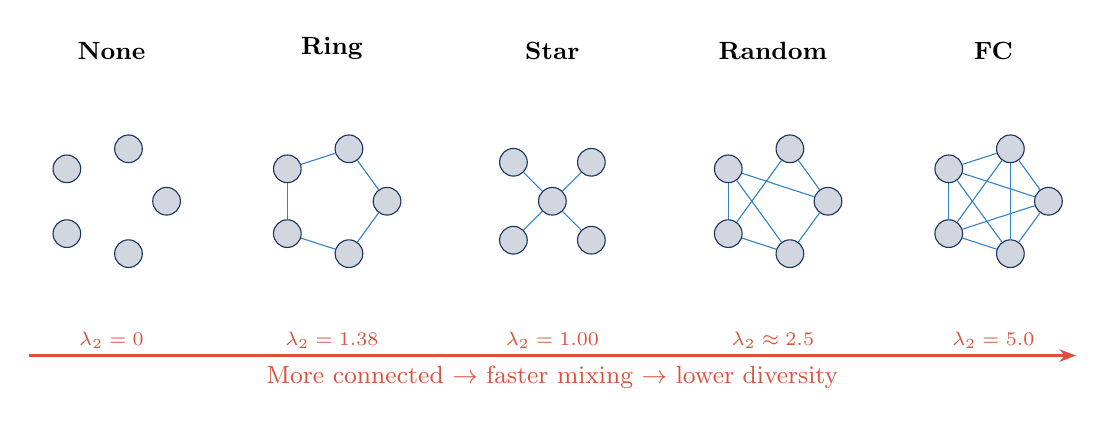
\begin{tikzpicture}[scale=0.7,
    node/.style={circle,draw=geccoBlue,fill=geccoBlue!20,
                 minimum size=10pt,inner sep=0pt},
    lbl/.style={font=\small\bfseries,above=12pt},
    lam/.style={font=\scriptsize\color{geccoHighlight},below=8pt}]

    % None
    \begin{scope}[xshift=0cm]
      \foreach \i in {1,...,5} {
        \node[node] (n\i) at ({72*\i-72}:1) {};
      }
      \node[lbl] at (0,1.8) {None};
      \node[lam] at (0,-1.8) {$\lambda_2 = 0$};
    \end{scope}

    % Ring
    \begin{scope}[xshift=4cm]
      \foreach \i in {1,...,5} {
        \node[node] (r\i) at ({72*\i-72}:1) {};
      }
      \foreach \i/\j in {1/2,2/3,3/4,4/5,5/1} {
        \draw[geccoAccent] (r\i) -- (r\j);
      }
      \node[lbl] at (0,1.8) {Ring};
      \node[lam] at (0,-1.8) {$\lambda_2 = 1.38$};
    \end{scope}

    % Star
    \begin{scope}[xshift=8cm]
      \node[node] (sc) at (0,0) {};
      \foreach \i in {1,...,4} {
        \node[node] (s\i) at ({90*\i-45}:1) {};
        \draw[geccoAccent] (sc) -- (s\i);
      }
      \node[lbl] at (0,1.8) {Star};
      \node[lam] at (0,-1.8) {$\lambda_2 = 1.00$};
    \end{scope}

    % Random
    \begin{scope}[xshift=12cm]
      \foreach \i in {1,...,5} {
        \node[node] (d\i) at ({72*\i-72}:1) {};
      }
      \draw[geccoAccent] (d1) -- (d2);
      \draw[geccoAccent] (d1) -- (d3);
      \draw[geccoAccent] (d2) -- (d4);
      \draw[geccoAccent] (d3) -- (d4);
      \draw[geccoAccent] (d3) -- (d5);
      \draw[geccoAccent] (d4) -- (d5);
      \draw[geccoAccent] (d1) -- (d5);
      \node[lbl] at (0,1.8) {Random};
      \node[lam] at (0,-1.8) {$\lambda_2 \approx 2.5$};
    \end{scope}

    % FC
    \begin{scope}[xshift=16cm]
      \foreach \i in {1,...,5} {
        \node[node] (f\i) at ({72*\i-72}:1) {};
      }
      \foreach \i in {1,...,5} {
        \foreach \j in {\i,...,5} {
          \draw[geccoAccent] (f\i) -- (f\j);
        }
      }
      \node[lbl] at (0,1.8) {FC};
      \node[lam] at (0,-1.8) {$\lambda_2 = 5.0$};
    \end{scope}

    % Arrow below
    \draw[-{Stealth[length=6pt]},thick,geccoHighlight]
      (-1.5,-2.8) -- (17.5,-2.8)
      node[midway,below,font=\small] {More connected $\to$ faster mixing $\to$ lower diversity};
  \end{tikzpicture}
  \end{center}
  \note{The five topologies ordered by algebraic connectivity lambda_2.
    Intuition: more connected = faster mixing = greater diversity erosion.}
\end{frame}

% ═══════════════════════════════════════════════════════
% SECTION 4: Main Results (5 min)
% ═══════════════════════════════════════════════════════
\section{Results}

% ── Slide 11: Universal Ordering ★ AHA MOMENT ────────
\begin{frame}{The Universal Ordering}
  \begin{center}
    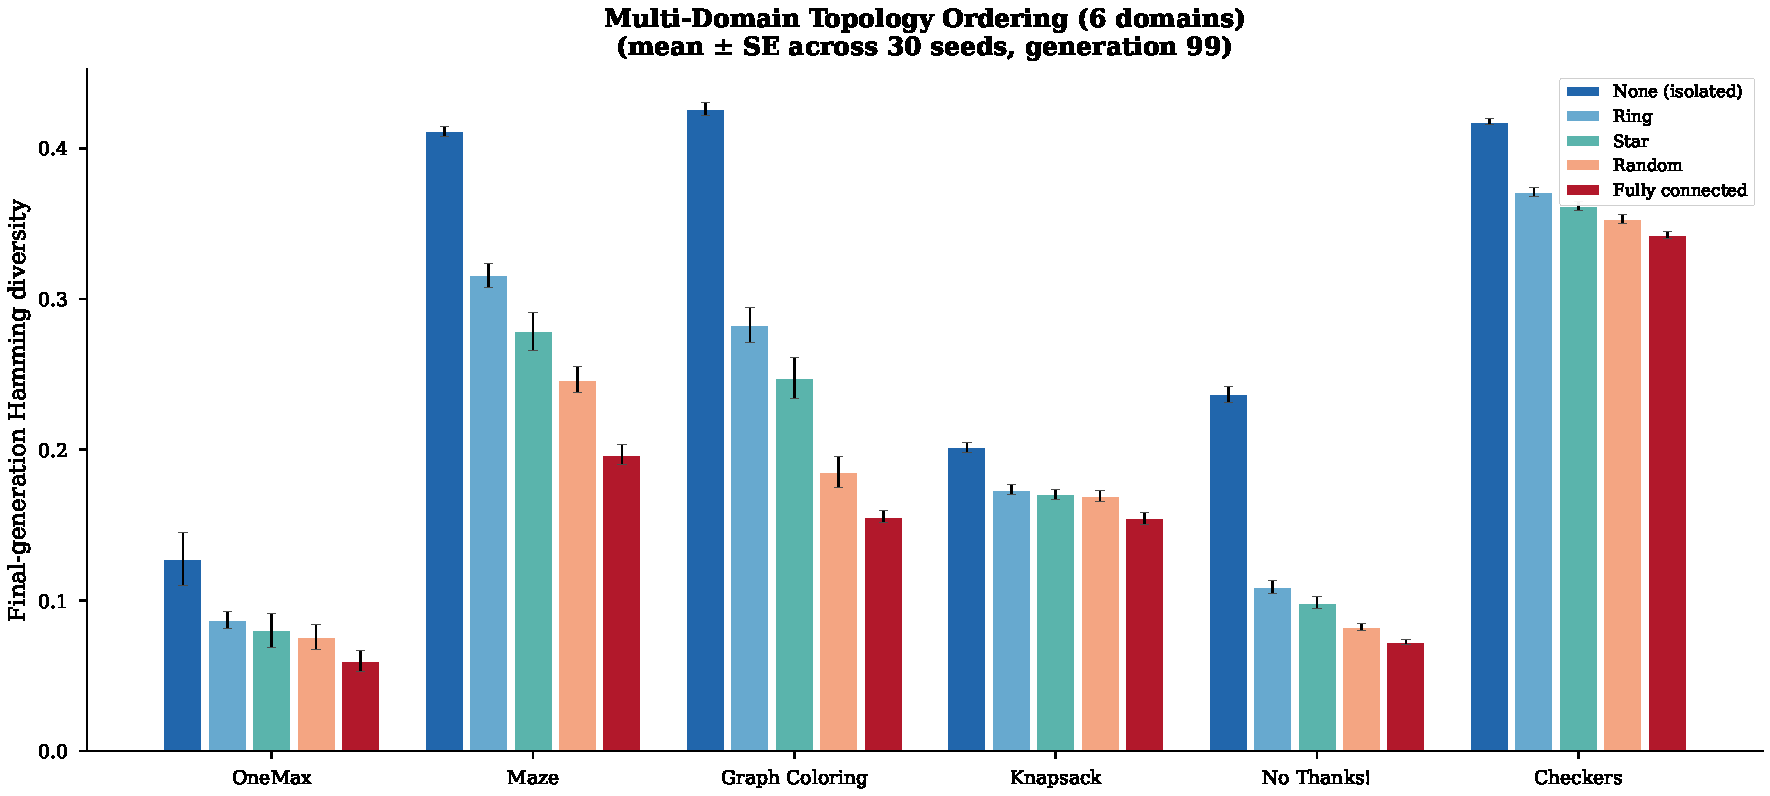
\includegraphics[width=0.8\textwidth]{multi_domain_topology_ordering.pdf}
  \end{center}

  \vspace{-4pt}
  \begin{center}
  \begin{tabular}{@{}cccc@{}}
    $W = 1.0$ & $p = 0.00008$ & $F_{\text{topo}} = 47.8$ & $F_{\text{domain}} = 0.13$ \\
    \scriptsize perfect concordance & \scriptsize highly significant &
    \scriptsize topology dominates & \scriptsize \alert{domain is noise}
  \end{tabular}
  \end{center}

  \note{THE central result. Pause here. Let it land.
    none > ring > star > random > FC in EVERY domain.
    Two-way ANOVA: topology F=47.8, domain F=0.13.
    Even No Thanks! (no fixed landscape) follows the ordering.}
\end{frame}

% ── Slide 12: Spectral Explanation ────────────────────
\begin{frame}{The Spectral Explanation}
  \begin{columns}[T]
    \column{0.55\textwidth}
    \begin{itemize}
      \item Ordering follows $\lambda_2$\\(algebraic connectivity)
      \item Smaller $\lambda_2$ $=$ slower mixing\\$=$ \alert{higher sustained diversity}
      \item None $\to$ ring: \textbf{35\% diversity drop}\\
            {\scriptsize (symmetry breaking dominates)}
      \item Subsequent steps: $\leq$ 9\% each
    \end{itemize}

    \vspace{8pt}
    \begin{center}
    {\small\itshape The first edge matters most.}
    \end{center}

    \column{0.45\textwidth}
    % Placeholder for lambda_2 vs diversity plot
    \begin{center}
      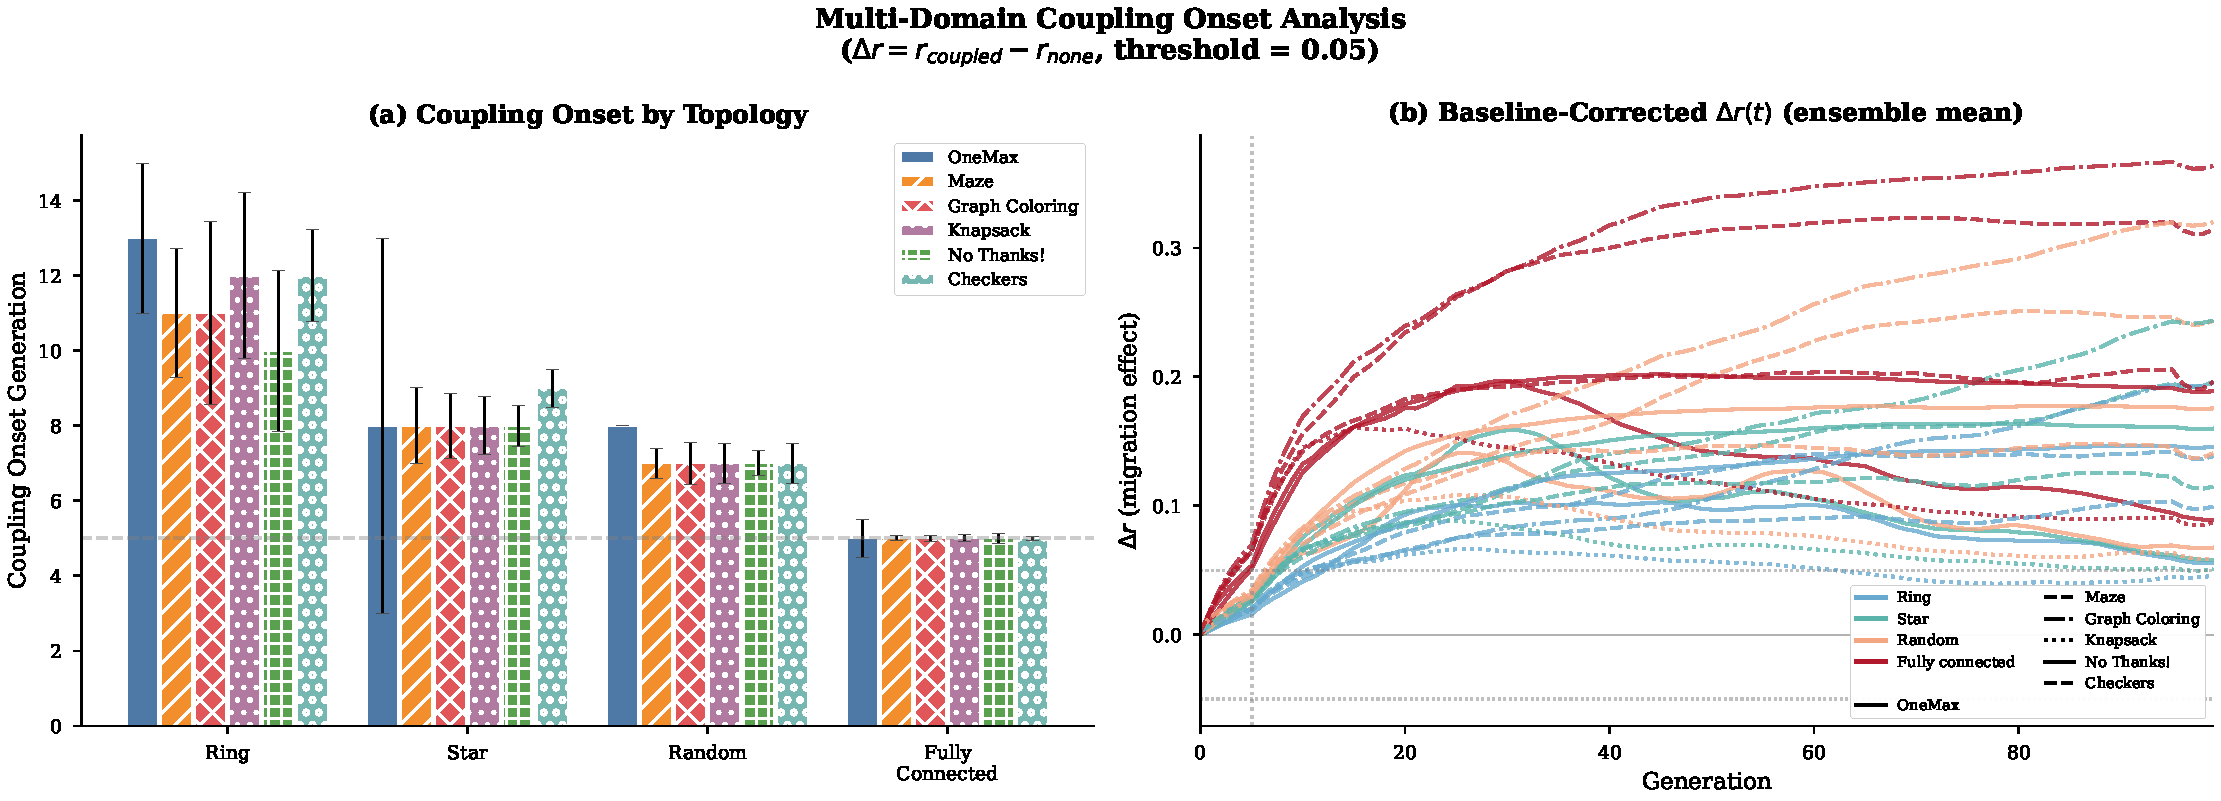
\includegraphics[width=\textwidth]{multi_domain_coupling_onset.pdf}
    \end{center}
  \end{columns}
  \note{Ordering follows lambda_2. The none-to-ring transition causes a 35\%
    diversity drop --- symmetry breaking dominates. After that, at most 9\% per step.}
\end{frame}

% ── Slide 13: Ring/Star Inversion ★ AHA MOMENT ───────
\begin{frame}{Falsifiable Prediction: Ring/Star Inversion}
  \begin{columns}[T]
    \column{0.5\textwidth}
    \begin{center}
      {\bfseries At $n = 5$}\\[4pt]
      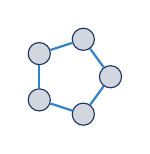
\begin{tikzpicture}[scale=0.5,
        node/.style={circle,draw=geccoBlue,fill=geccoBlue!20,
                     minimum size=8pt,inner sep=0pt}]
        \foreach \i in {1,...,5} {
          \node[node] (r\i) at ({72*\i-72}:1) {};
        }
        \foreach \i/\j in {1/2,2/3,3/4,4/5,5/1} {
          \draw[geccoAccent,thick] (r\i) -- (r\j);
        }
      \end{tikzpicture}\\[4pt]
      $\lambda_2(\text{ring}) = 1.38 > 1.0 = \lambda_2(\text{star})$\\[4pt]
      {\small Hard to distinguish}\\
      $p = 0.14$ {\scriptsize (as predicted)}
    \end{center}

    \column{0.5\textwidth}
    \begin{center}
      {\bfseries At $n = 7$}\\[4pt]
      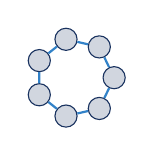
\begin{tikzpicture}[scale=0.5,
        node/.style={circle,draw=geccoBlue,fill=geccoBlue!20,
                     minimum size=8pt,inner sep=0pt}]
        \foreach \i in {1,...,7} {
          \node[node] (r\i) at ({360/7*\i}:1) {};
        }
        \foreach \i in {1,...,6} {
          \pgfmathtruncatemacro{\j}{\i+1}
          \draw[geccoAccent,thick] (r\i) -- (r\j);
        }
        \draw[geccoAccent,thick] (r7) -- (r1);
      \end{tikzpicture}\\[4pt]
      $\lambda_2(\text{ring}) = 0.75 \alert{<} 1.0 = \lambda_2(\text{star})$\\[4pt]
      {\small\bfseries Inequality reverses!}\\
      Ring: $0.387$ vs Star: $0.336$\\
      $p = 6.6 \times 10^{-5}$ {\scriptsize\color{geccoGreen} \checkmark{} confirmed}
    \end{center}
  \end{columns}

  \vfill
  \begin{center}
    {\small\alert{Theory predicts, experiment confirms.} Not post-hoc --- \textbf{novel prediction.}}
  \end{center}
  \note{AHA MOMENT. At n=5, ring and star have similar lambda_2 --- hard to distinguish (p=0.14).
    At n=7, the inequality reverses --- ring should clearly beat star. Confirmed: p = 6.6e-5.
    This is science: the theory makes novel predictions.}
\end{frame}

% ── Slide 14: Scope Condition ─────────────────────────
\begin{frame}{Scope Condition: Sorting Networks}
  \begin{center}
    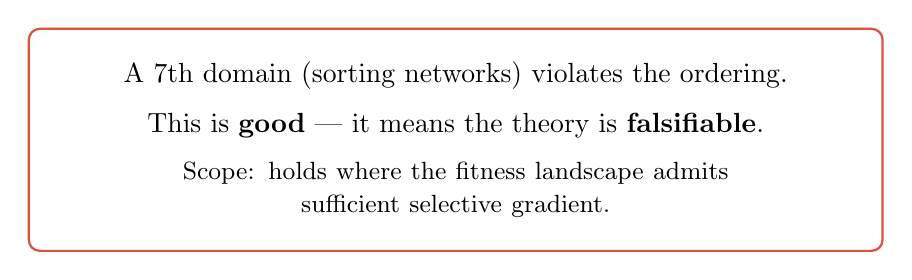
\begin{tikzpicture}
      \node[draw=geccoHighlight,thick,rounded corners,inner sep=12pt,
            text width=10cm,align=center]
        {A 7th domain (sorting networks) \alert{violates} the ordering.\\[6pt]
         This is \textbf{good} --- it means the theory is \textbf{falsifiable}.\\[6pt]
         {\small Scope: holds where the fitness landscape admits\\sufficient selective gradient.}};
    \end{tikzpicture}
  \end{center}
  \note{Sorting networks violate the ordering. This shows the theory is falsifiable.
    Scope: holds where fitness landscape admits sufficient selective gradient.
    Don't dwell --- shows scientific honesty.}
\end{frame}

% ═══════════════════════════════════════════════════════
% SECTION 5: Diversity Fingerprints (3 min)
% ═══════════════════════════════════════════════════════
\section{Diversity Fingerprints}

% ── Slide 15: Four Strategy Compositions ──────────────
\begin{frame}{Four Strategy Compositions}
  {\small Same operators, different composition patterns:}

  \vspace{8pt}
  \begin{columns}[T]
    \column{0.25\textwidth}
    \centering
    {\bfseries Generational}\\[4pt]
    {\scriptsize iterate($f$)}\\[4pt]
    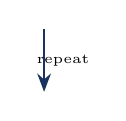
\begin{tikzpicture}[scale=0.4]
      \draw[-{Stealth},thick,geccoBlue] (0,0) -- (0,-2);
      \node[font=\tiny] at (0.6,-1) {repeat};
    \end{tikzpicture}

    \column{0.25\textwidth}
    \centering
    {\bfseries Hourglass}\\[4pt]
    {\scriptsize 3 phases}\\[4pt]
    
\begin{tikzpicture}[scale=0.4]
      \draw[-{Stealth},thick,geccoBlue] (0,0) -- (0,-0.7);
      \draw[-{Stealth},thick,geccoHighlight] (0,-0.7) -- (0,-1.4);
      \draw[-{Stealth},thick,geccoGreen] (0,-1.4) -- (0,-2);
    \end{tikzpicture}

    \column{0.25\textwidth}
    \centering
    {\bfseries Island}\\[4pt]
    {\scriptsize parallel + migrate}\\[4pt]
    
\begin{tikzpicture}[scale=0.4]
      \draw[-{Stealth},thick,geccoBlue] (-0.5,0) -- (-0.5,-2);
      \draw[-{Stealth},thick,geccoBlue] (0.5,0) -- (0.5,-2);
      \draw[{Stealth}-{Stealth},thick,geccoAccent] (-0.3,-1) -- (0.3,-1);
    \end{tikzpicture}

    \column{0.25\textwidth}
    \centering
    {\bfseries Adaptive}\\[4pt]
    {\scriptsize conditional switch}\\[4pt]
    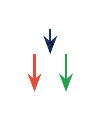
\begin{tikzpicture}[scale=0.4]
      \draw[-{Stealth},thick,geccoBlue] (0,0) -- (0,-0.8);
      \draw[-{Stealth},thick,geccoHighlight] (-0.5,-0.8) -- (-0.5,-2);
      \draw[-{Stealth},thick,geccoGreen] (0.5,-0.8) -- (0.5,-2);
      \node[font=\tiny] at (0,-0.6) {?};
    \end{tikzpicture}
  \end{columns}
  \note{Same operators composed in four different patterns.
    Generational (iterate), Hourglass (3 phases), Island (parallel + migration),
    Adaptive (conditional switch on plateau detection).}
\end{frame}

% ── Slide 16: Fingerprint Chart ★ AHA MOMENT ─────────
\begin{frame}{Diversity Fingerprints}
  \begin{center}
    \includegraphics[width=0.85\textwidth]{gecco_two_panel.pdf}
  \end{center}
  \vspace{-4pt}
  \begin{center}
    {\small Same operators. \alert{18$\times$ spread} in final diversity.\\
    \textbf{Composition is everything.}}
  \end{center}
  \note{AHA MOMENT. Same operators, 18x difference in final diversity.
    Monotonic decline (generational), spike-crash-rebound (hourglass),
    stable maintenance (island), spike-then-collapse (adaptive).
    Composition determines the trajectory shape.}
\end{frame}

% ── Slide 17: Fingerprints Stable Across Domains ─────
\begin{frame}{Fingerprints Are Stable Across Domains}
  \begin{columns}[T]
    \column{0.6\textwidth}
    \begin{itemize}
      \item Patterns replicate across\\maze, graph coloring, knapsack
      \item Shape determined by\\
            \alert{composition}, not landscape
      \item You can predict diversity trajectory\\
            from composition structure alone
    \end{itemize}

    \column{0.4\textwidth}
    \begin{center}
      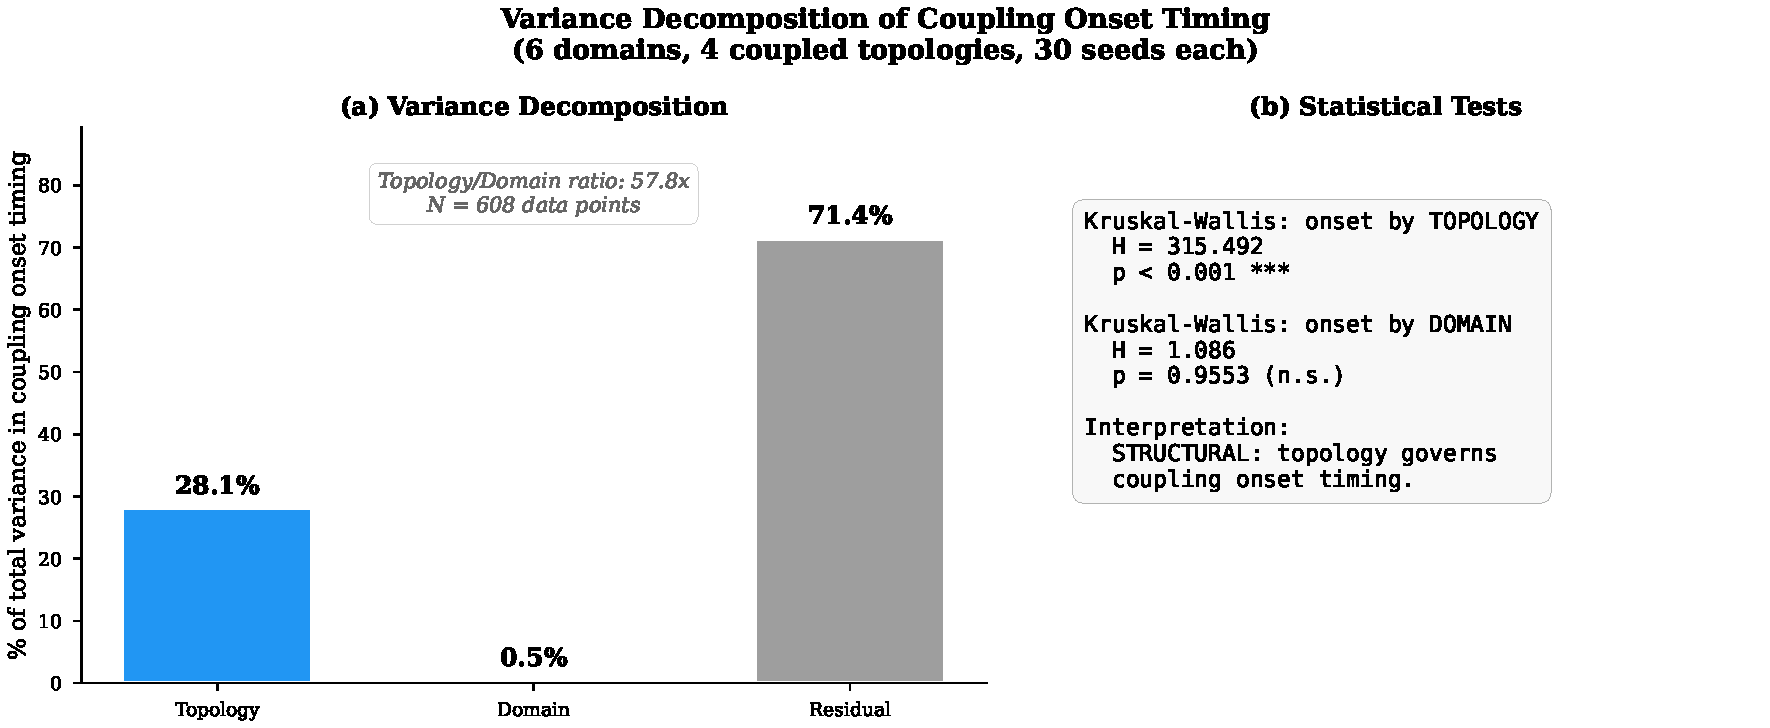
\includegraphics[width=\textwidth]{multi_domain_variance_decomposition.pdf}
    \end{center}
  \end{columns}
  \note{Fingerprint patterns replicate across all domains. The shape is determined
    by composition, not landscape. Implication: predict diversity trajectory
    from composition structure alone.}
\end{frame}

% ═══════════════════════════════════════════════════════
% SECTION 6: Practical Implications + Conclusion (2 min)
% ═══════════════════════════════════════════════════════
\section{Implications}

% ── Slide 18: Three Recommendations ──────────────────
\begin{frame}{Three Recommendations for Practitioners}
  \begin{enumerate}
    \item \textbf{Prefer ring/mesh over star}\\
          {\small $\beta_1 \geq 1$ avoids the composition-tax singularity}

    \vspace{8pt}
    \item \textbf{Monitor $\lambda_2$, not diversity directly}\\
          {\small Early warning signal, cheap to compute from topology alone}

    \vspace{8pt}
    \item \textbf{Add cycle-closing edges}, don't increase migration rate\\
          {\small Changes topology structure, not just coupling strength}
  \end{enumerate}

  \vspace{10pt}
  \begin{center}
  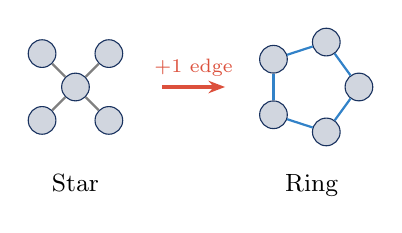
\begin{tikzpicture}[scale=0.5,
    node/.style={circle,draw=geccoBlue,fill=geccoBlue!20,
                 minimum size=10pt,inner sep=0pt}]
    % Star
    \node[node] (sc) at (0,0) {};
    \foreach \i/\a in {1/45,2/135,3/225,4/315} {
      \node[node] (s\i) at (\a:1.2) {};
      \draw[gray,thick] (sc) -- (s\i);
    }
    \node[below=8pt,font=\small] at (0,-1.4) {Star};

    % Arrow
    \draw[-{Stealth[length=6pt]},very thick,geccoHighlight] (2.2,0) -- (3.8,0)
      node[midway,above,font=\scriptsize] {+1 edge};

    % Ring
    \begin{scope}[xshift=6cm]
      \foreach \i in {1,...,5} {
        \node[node] (r\i) at ({72*\i-72}:1.2) {};
      }
      \foreach \i/\j in {1/2,2/3,3/4,4/5,5/1} {
        \draw[geccoAccent,thick] (r\i) -- (r\j);
      }
      \node[below=8pt,font=\small] at (0,-1.4) {Ring};
    \end{scope}
  \end{tikzpicture}
  \end{center}
  \note{Three practical recommendations.
    1. Prefer ring/mesh over star.
    2. Monitor lambda_2, not diversity directly.
    3. Add cycle-closing edges rather than increasing migration rate.}
\end{frame}

% ── Slide 19: Summary + Future Work ──────────────────
\begin{frame}{Summary}
  \begin{columns}[T]
    \column{0.55\textwidth}
    \begin{itemize}
      \item \textbf{Composition determines diversity}\\
            {\small empirically, across 6 domains}
      \item \textbf{Universal topology ordering}\\
            {\small $W = 1.0$, explained by $\lambda_2$}
      \item \textbf{Diversity fingerprints} are properties\\
            of composition patterns
      \item \textbf{Falsifiable} predictions confirmed
    \end{itemize}

    \column{0.45\textwidth}
    \begin{center}
    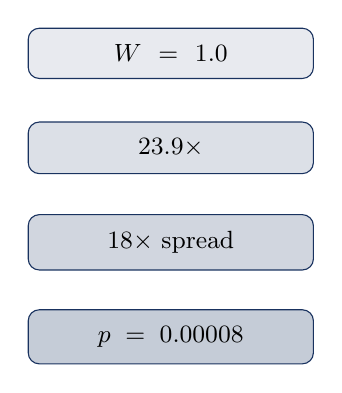
\begin{tikzpicture}[
      stat/.style={draw=geccoBlue,rounded corners,inner sep=6pt,
                   text width=3.2cm,align=center,font=\small}]
      \node[stat,fill=geccoBlue!10] at (0,0) {$W = 1.0$};
      \node[stat,fill=geccoBlue!15] at (0,-1.2) {$23.9\times$};
      \node[stat,fill=geccoBlue!20] at (0,-2.4) {$18\times$ spread};
      \node[stat,fill=geccoBlue!25] at (0,-3.6) {$p = 0.00008$};
    \end{tikzpicture}
    \end{center}
  \end{columns}

  \vspace{8pt}
  {\small\color{gray} Future: larger populations, longer runs, heterogeneous island strategies}
  \note{Summary with key numbers. Future work directions.}
\end{frame}

% ── Slide 20: Thank You ──────────────────────────────
{
\setbeamercolor{background canvas}{bg=geccoBlue}
\begin{frame}[plain]
  \vfill
  \begin{center}
    {\Huge\bfseries\color{white} Thank You}\\[16pt]
    {\color{geccoAccent}\large Questions?}\\[24pt]
    {\small\color{white}
      Robin Langer \quad\textbar\quad langer.robin@gmail.com\\[4pt]
      \texttt{github.com/RaggedR/categorical-evolution}}\\[16pt]
    {\small\color{gray!60}\itshape
      ``How you wire your islands matters more than what you evolve''}
  \end{center}
  \vfill
\end{frame}
}

\end{document}
